\Chapter{Tervezés}

A szimulációs környezet megfelelő működéséhez el kell tárolnunk az ágensek és a mapot összeállító blockok adatait.
Ennek a megvalósításához szükséges leírni mely adatokat kell eltárolnunk és adatmodelleket készítése is elegedhetetlen az átláthatóságért.

\section{Adatmodellek}

\subsection{Tárolandó elemek}

\begin{itemize}
    \item Room

    \begin{itemize}
        \item RoomID
    \end{itemize}

    \item Block

    \begin{itemize}
        \item BlockID
        \item X
        \item Y
    \end{itemize}

    \item RoomObjects

    \begin{itemize}
        \item RoomObjectsID
    \end{itemize}

    \item Agent

    \begin{itemize}
        \item AgentID
        \item AgentFaction
    \end{itemize}

    \item AgentType

    \begin{itemize}
        \item AgentType
        \item Desc
    \end{itemize}

    \item Stat

    \begin{itemize}
        \item STR
        \item VIT
        \item EVA
        \item ACC
    \end{itemize}

    \item Inventory

    \begin{itemize}
        \item Slots
    \end{itemize}

    \item Item

    \begin{itemize}
        \item ItemID
        \item ItemName
        \item Quantity
        \item MaxQuantity
    \end{itemize}

    \item ItemType

    \begin{itemize}
        \item ItemType
        \item Desc
    \end{itemize}

    \item ObjectObstructingMovement

    \begin{itemize}
        \item OOMID
    \end{itemize}

    \item ObjObsMovType

    \begin{itemize}
        \item OOMType
        \item Desc
    \end{itemize}

    \item Effect

    \begin{itemize}
        \item EffectID
        \item EffectTime
    \end{itemize}

    \item EffectType

    \begin{itemize}
        \item EffectType
        \item Desc
    \end{itemize}

\end{itemize}

\subsection{ER adatmodell}

\nameref{fig:Szemantikai modell}

\subsection{Szemantikai adatmodell egyedei}

A szemantikai adatmodellben összesen 12 egyed szerepel, amelyek a következők:

\begin{itemize}
    \item Room
    \item Block
    \item RoomObjects
    \item OOM
    \item OOMType
    \item Item
    \item ItemType
    \item Agent
    \item AgentType
    \item Stat
    \item Effect
    \item EffectType
\end{itemize}

\subsection{Egyed tulajdonságok}

\begin{itemize}

    \item Room egyed tulajdonságai:
    
    \begin{itemize}
        \item RoomID: A szobák egyedi azonosítója, integer érték.
    \end{itemize}

    \item Block egyed tulajdonságai:
    
    \begin{itemize}
        \item BlockID: A blokkok egyedi azonosítója, integer érték.
        \item X: Az adott blokkhoz tartozó X koordináta, integer érték.
        \item Y: Az adott blokkhoz tartozó Y koordináta, integer érték.
    \end{itemize}

    \item RoomObjects egyed tulajdonságai:
    
    \begin{itemize}
        \item RoomObjectsID: A blokkon szereplő Objektum egyedi azonosítója, integer érték.
    \end{itemize}

    \item OOM egyed tulajdonságai:
    
    \begin{itemize}
        \item OOMID: Mozgást kizárló objektum egyedi azonosítója, integer érték.
    \end{itemize}

    \item OOMType egyed tulajdonságai:
    
    \begin{itemize}
        \item OOMType: Mozgást kizárló objektum neve, String érték.
        \item Desc: Mozgást kizárló objektum leírása.
    \end{itemize}

    \item Item egyed tulajdonságai:
    
    \begin{itemize}
        \item ItemID: A tárgy egyedi azonosítója, integer érték. 
        \item ItemName: A tárgy neve, String érték.
        \item Quantity: A tárgy darabszáma, integer érték.
        \item MaxQuantity: A tárgy maximum darabszáma, integer érték.
    \end{itemize}

    \item ItemType egyed tulajdonságai:
    
    \begin{itemize}
        \item ItemTypeID: A tárgy típus egyedi azonosítója, integer érték.
        \item ItemTypeName: A tárgy típusának a neve, String érték.
        \item Desc: A tárgy típusának leírása.
    \end{itemize}

    \item Agent egyed tulajdonságai:
    
    \begin{itemize}
        \item AgentID: Az ágens egyedi azonosítója, integer érték.
        \item AgentFaction: Az ágens frakcióját tartalmazza, String érték.
    \end{itemize}

    \item AgentType egyed tulajdonságai:

    \begin{itemize}
        \item AgentTypeID: Az ágens típus egyedi azonosítója, integer érték.
        \item AgentTypeName: Az ágens típusának a neve, String érték.
        \item Desc: Az ágens típusának a leírása.
    \end{itemize}

    \item Stat egyed tulajdonságai:

    \begin{itemize}
        \item StatID: Statisztika egyedi azonosítója, integer érték.
        \item STR: A STR érték mennyiségét tartalmazza, integer érték.
        \item VIT: A VIT érték mennyiségét tartalmazza, integer érték.
        \item EVA: A EVA érték mennyiségét tartalmazza, integer érték.
        \item ACC: A ACC érték mennyiségét tartalmazza, integer érték.
    \end{itemize}

    \item Effect egyed tulajdonságai:

    \begin{itemize}
        \item EffectID: Effekt egyedi azonosítója, integer érték.
        \item EffectTime: Effekt hátralévő ideje körökben, integer érték.
    \end{itemize}

    \item EffectType egyed tulajdonságai:

    \begin{itemize}
        \item EffectTypeID: Az effekt típus egyedi azonosítója, integer érték.
        \item EffectTypeName: Az effekt típus neve, String érték.
        \item Desc: Az effekt típus leírása, String érték.
    \end{itemize}

    \item Inventory egyed tulajdonságai:
    \item 
    \begin{itemize}
        \item Slots: Az inventoryban maximális helyet meghatározó érték, integer érték.
    \end{itemize}

\end{itemize}

\subsection{Egyedek közöti kapcsolat}

\begin{itemize}
    \item Agent és AgentType egyedek között egy a többhöz kapcsolat van, mivel egy ágenshez egy ágens típus tartozhat, de egy ágens típus több ágenshez is tartozhat.
    \item Agent és Stat egyedek között egy az egyhez kapcsolat van, mivel egy ágenshez szigorúan egy statisztika ablak tartozhat és egy statisztika ablakhoz csak egy ágens tartozhat.
    \item Agent és Tárgy egyedek között több a többhöz kapcsolat van, mivel egy ágenshez tartozhat több tárgy, ahogyan egy tárgy tartozhat több ágenshez is.
    \item Item és ItemType egyedek között egy a többhöz kapcsolat van, mivel egy tárgyhoz egy tárgy típus tartozhat, de egy tárgy típus több tárgyhoz is tartozhat.
    \item Room és Block egyedek között egy a többhöz kapcsolat van, mivel egy szobához több block tartozik, de egy blockhoz nem tartozhat több szoba.
    \item Agent és Block egyedek között egy az egy kapcsolat van, mivel egy blockhoz csak egy ágens tartozhat, egy ágenshez szintén csak egy block tartozhat.
    \item Agent és Effect egyedek között több a többhöz kapcsolat van, mivel egy ágenshez tartozhat több effekt, ahogy egy effekt is tartozhat több ágenshez.
    \item Effect és Type egyedek között egy a több kapcsolat van, mivel egy effekt csak egy effekt típus tartozhat, de egy effekt típus tartozhat több effekthez.
    \item Effect és Block egyedek között több a több kapcsolat van, mivel egy effekt tartozhat több blockhoz, de egy blokkhoz is tartozhat több effekt.
    \item Block és RoomObjects egyedek között egy a többhöz kapcsolat van, mivel egy blockhoz csak egy RoomObject tartozhat, de egy RoomObject tartozhat több blockhoz.
    \item RoomObject és Item egyedek között egy a több kapcsolat van, mivel egy RoomObjectshez csak egy tárgy tartozhat, de egy Tárgyhoz tartozhat több RoomObjects.
    \item RoomObject és OOM egyedek között egy a több kapcsolat van, mivel egy RoomObjectshez csak egy OOM tartozhat, de egy OOM tartozhat több RoomObjects.
    \item RoomObject és OOMType egyedek között egy a több kapcsolat van, mivel egy OOMhez csak egy OOM típus tartozhat, de egy OOM típushoz tartozhat több OOM.
    \item Effect és Block egyedek között több a több kapcsolat van, mivel egy effekt tartozhat több blockhoz, ahogy egy blockhoz is tartozhat több effekt.

\end{itemize}

\section{Relációs adatmodell}

\nameref{fig:Relációs modell}

\subsection{Szemantikai adatmodell konvertálása relációs modellre}



\begin{figure}[!ht]
	\centering
	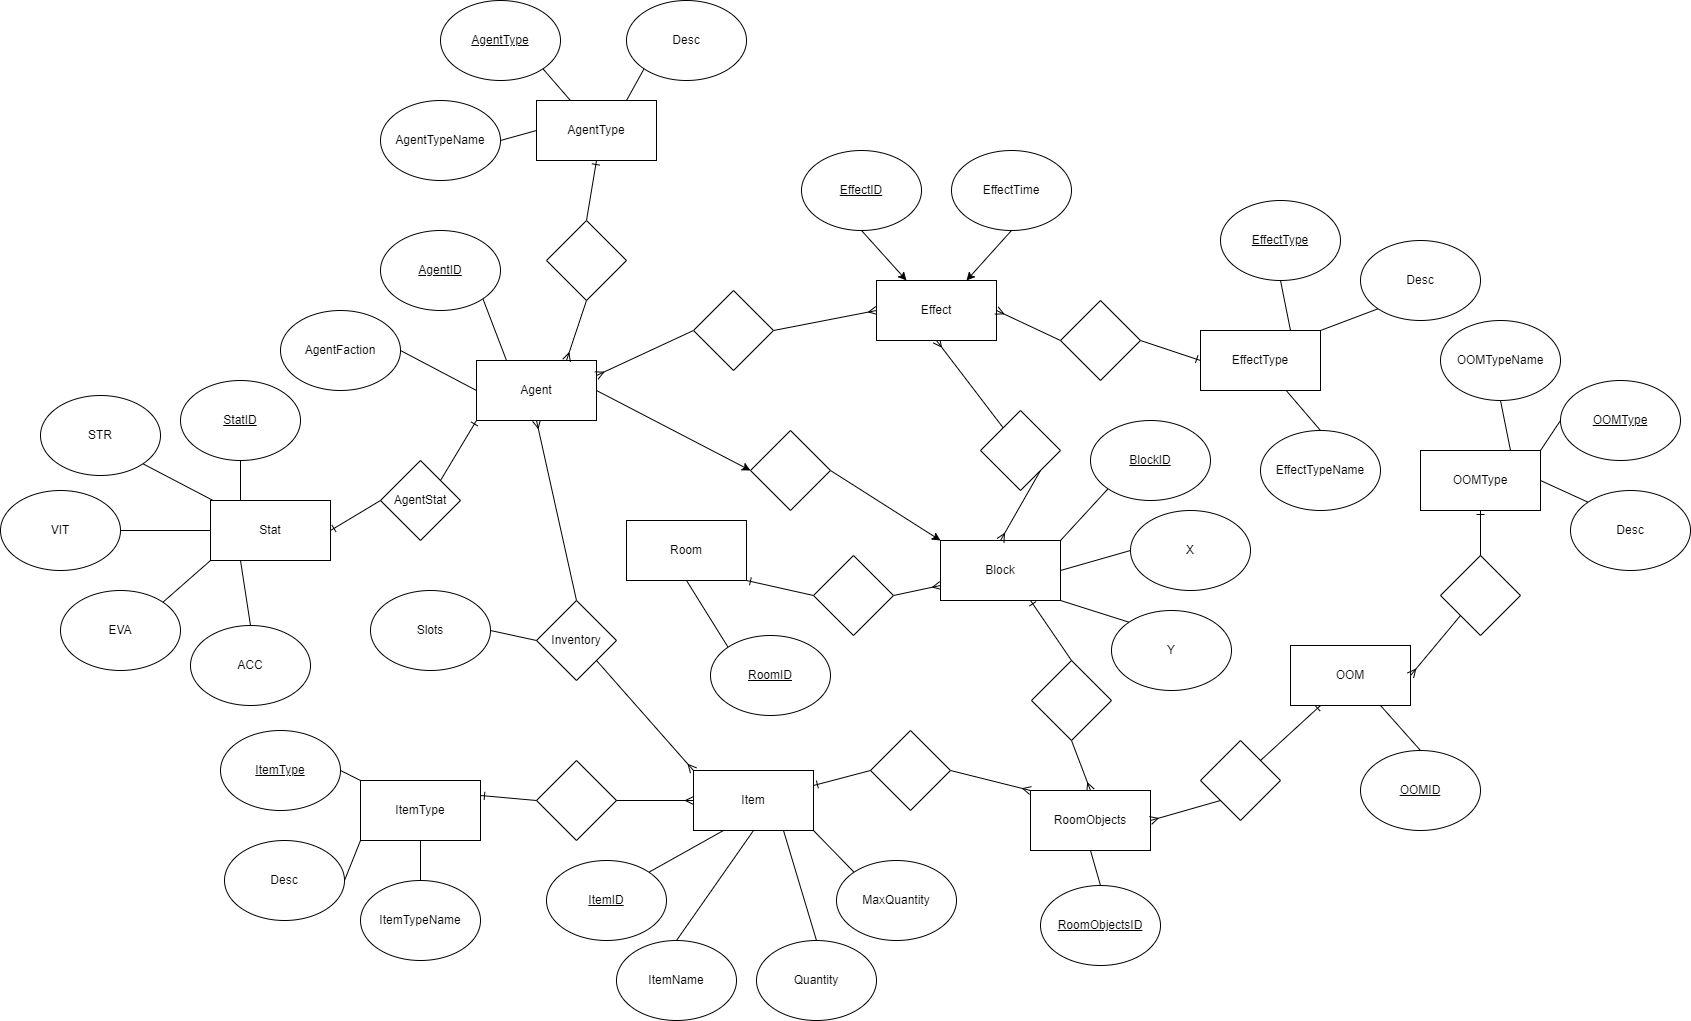
\includegraphics[scale=0.25]{images/szemantikaimodel6.drawio.png}
	\caption{Szemantikai modell}
	\label{fig:Szemantikai modell}
\end{figure}

\begin{figure}[!ht]
	\centering
	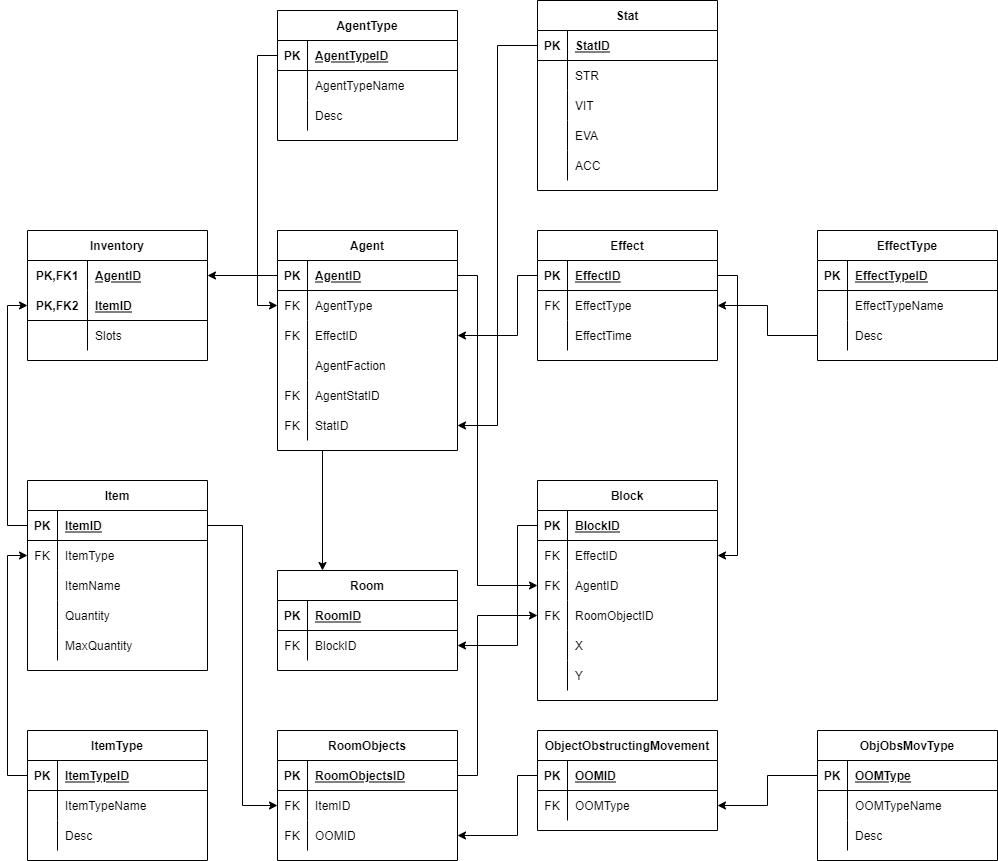
\includegraphics[scale=0.35]{images/relaciosadatmodel6.drawio.png}
	\caption{Relációs modell}
	\label{fig:Relációs modell}
\end{figure}

\iffalse
Itt kezdődik a dolgozat lényegi része, úgy értve, hogy a saját munka bemutatása.
Jellemzően ebben szerepelni szoktak blokkdiagramok, a program struktúrájával foglalkozó leírások.
Ehhez célszerű UML ábrákat (például osztály- és szekvenciadiagramokat) használni.

Amennyiben a dolgozat inkább kutatás jellegű, úgy itt lehet konkretizálni a kutatási módszertant, a kutatás tervezett lépéseit, az indoklást, hogy mit, miért és miért pont úgy érdemes csinálni, ahogyan az a későbbiekben majd részletezésre kerül.

Ebben a fejezetben az implementáció nem kell, hogy túl nagy szerepet kapjon.
Ez még csak a tervezési fázis.
(Nyilván ha olyan a téma, hogy magának az implementációnak a módjával foglalkozik, adott formális nyelvet mutat be, úgy a kódpéldákat már innen sem lehet kihagyni.)

\Section{Táblázatok}

Táblázatokhoz a \texttt{table} környezetet ajánlott használni.
Erre egy minta \aref{tab:minta}. táblázat.
A hivatkozáshoz az egyedi \texttt{label} értéke konvenció szerint \texttt{tab:} prefixszel kezdődik.

\begin{table}[h]
\centering
\caption{Minta táblázat. A táblázat felirata a táblázat felett kell legyen!}
\label{tab:minta}
\begin{tabular}{l|c|c|}
a & b & c \\
\hline
1 & 2 & 3 \\
4 & 5 & 6 \\
\hline
\end{tabular}
\end{table}

\Section{Ábrák}

Ábrákat a \texttt{figure} környezettel lehet használni.
A használatára egy példa \aref{fig:cimer}. ábrán látható.
Az \texttt{includegraphics} parancsba 
Az ábrák felirata az ábra alatt kell legyen.
Az ábrák hivatkozásához használt nevet konvenció szerint \texttt{fig:}-el célszerű kezdeni.

\begin{figure}[h]
\centering

\includegraphics[scale=0.3]{images/me_logo.png}
\caption{A Miskolci Egyetem címere.}
\label{fig:cimer}
\end{figure}

\Section{További környezetek}

A matematikai témájú dolgozatokban szükség lehet tételek és bizonyításaik megadására.
Ehhez szintén vannak készen elérhető környezetek.

\begin{definition}
Ez egy definíció
\end{definition}

\begin{lemma}
Ez egy lemma
\end{lemma}

\begin{theorem}
Ez egy tétel
\end{theorem}

\begin{proof}
Ez egy bizonyítás
\end{proof}

\begin{corollary}
Ez egy tétel
\end{corollary}

\begin{remark}
Ez egy megjegyzés
\end{remark}

\begin{example}
Ez egy példa
\end{example}
\fi